\documentclass[a4paper,11pt]{report}

\usepackage[latin1]{inputenc}
\usepackage{amsmath}
\usepackage{amsfonts}
\usepackage{amssymb}
\usepackage{graphicx}
\usepackage[spanish]{babel}
\usepackage{fancyhdr}
\usepackage{indentfirst}
\usepackage{verbatim}
\usepackage{alltt}
\usepackage{hyperref}
\usepackage[left=3cm,top=3cm,right=2.5cm,bottom=2.5cm]{geometry}

% style for code citation
\newenvironment{code}
	{\begin{quote}\begin{alltt}}
	{\end{alltt}\end{quote}}

% fast commands to write system components names
\newcommand{\plfs}{\textit{plfs }}
\newcommand{\kplfs}{\textit{kplfs }}
\newcommand{\uplfs}{\textit{uplfs }}
\newcommand{\dpld}{\textit{dpld }}
\newcommand{\pldb}{\textit{pldb }}
\newcommand{\umcc}{\textit{umcc }}
\newcommand{\umc}{\textit{umc }}
\newcommand{\umcr}{\textit{umcr }}
\newcommand{\dplc}{\textit{dplc }}
\newcommand{\famon}{\textit{fam }}

% 4 levels of enumeration and indexing
\setcounter{secnumdepth}{4}
\setcounter{tocdepth}{4}

% Title Page
\author{
  Jonathan Mart� Fraiz \\
  \textit{jonathan.marti@upc.edu}
  \and
  Llu�s Vilanova Garc�a \\
  \textit{xscript@gmx.net}
}

\title{
  \textbf{
  Desplegamiento Paralelitzado \\
  de Aplicaciones en PlanetLab \\
  a Trav�s del Sistema de Ficheros
  }
}


\begin{document}

\maketitle

\tableofcontents

% Headers
\pagestyle{fancy}
%\fancyhf{} % delete all adjustments
% From here on, fancyhead is used to configure the header, fancyfoot for the
% footer
% Justification: C=centered, R=right, L=left, (nothing)=LRC
% Page: O=odd, E=even, (nothing)=OE
\fancyhead[]{}  % chapter number
\fancyhead[L]{\leftmark}  % chapter number
%\fancyhead[R]{\thepage} % page number
% Modifies the width of the header and footer lines
\renewcommand{\chaptermark}[1]{
	\markboth{\chaptername\  \thechapter. #1}{}
}
\renewcommand{\headrulewidth}{0.4pt}

\chapter{Qu� y porqu� lo queremos hacer?}

Tanto la documentaci�n como la implementaci�n se encuentran disponibles en la
p�gina del proyecto \cite{PLFS}, que basa su idea inicial en la propuesta de
\cite{ParPipelinedDist}.

Cabe notar que, como inicialmente nos centraremos en las operaciones de
despliegue, siempre que nos refiramos a \plfs, s�lo estaremos haciendo
referencia, realmente, al subconjunto dedicado al despliegue.

El proyecto pretende juntar b�sicamente dos conceptos con tal de conseguir dos
grandes objetivos:



\section{Facilidad de uso}

A trav�s de una interf�cie que todo el mundo ya conozca y necesite un m�nimo
de aprendizaje y permita un f�cil desarrollo de aplicaciones de m�s alto
nivel.

Este objetivo pretende conseguirse a trav�s de la implementaci�n de un sistema
de ficheros, con una estructura a�n por determinar, pero que permita desplegar
una aplicaci�n de una forma tan f�cil como copiar un fichero en un directorio
concreto, evento que disparar�a el sistema de distribuci�n de ficheros.



\section{Eficiencia en la transferencia de ficheros}

Como la aplicaci�n a desplegar necesita ser copiada a todos los nodos de un
slice, no basta con copiarla directamente a un sistema de ficheros "en red"
convencional, puesto que se enviar�a a un punto central y luego todos los
nodos, al arrancar el servicio, leer�an a la vez el programa para poder
ponerlo en marcha, saturando innecesariamente la red.

Para �ste fin, la idea de una distribuci�n multicast es ideal, ya que
permitir�a ahorrar al m�ximo el ancho de banda, permitiendo un despliegue
en paralelo y evitando al m�ximo las aglomeraciones de datos innecesarias.

Como la mayor�a de routers de Internet no soportan el enrutamiento multicast,
es por eso que har�a falta un servicio en modo usuario que se encargara de
hacer �sta distribuci�n.


\chapter{Arquitectura del sistema}

\textbf{\textit{En este cap�tulo comentamos la arquitectura general del
sistema, los componentes necesarios, el sistema de ficheros y las operaciones
que debe implementar.}}



\section{Componentes}

En este apartado mostraremos un esquema inicial de los principales
componentes que necesitar�a el sistema presentado (figura
\ref{fig:arquitectura}):

\begin{description}
	\item [\kplfs:] PlanetLab File System (Kernel-mode Side)\\
		Componente del sistema de ficheros para PlanetLab que funciona dentro
		del n�cleo de Linux.
		\\
		Este componente, puede en realidad ser varios, cada uno dando
		unos servicios concretos (uno para el desplegamiento, uno para
		monitorizaci�n, \ldots).

	\item [\uplfs:] PlanetLab File System (User-mode Side)\\
		Componente del sistema de ficheros para PlanetLab que funciona en modo
		usuario.
		\\
		Este componente en realidad hace de intermediario entre el
		propio sistema de ficheros (es decir, el n�cleo) y los
		componentes que permiten realizar las funcionalidades y
		comunicaciones (en nuestro caso, ser�a \dpld).

	\item [\dpld:] Deployer Daemon\\
		Componente encargado de mandar las �rdenes de desplegamiento y
		mantener actualizada la visi�n que tiene el usuario sobre los
		slices de desplegamiento.

	\item [\pldb :] PlanetLab Data Base (para obtener inicialmente la lista
		de nodos de un slice)\\
		Componente para obtener datos de PlanetLab Central (PLC).

	\item [\umcc :] User-mode Multicast Client\\
		Componente encargado de las comunicaciones entre un sistema cualquiera
		y la red multicast.

	\item [\umcr :] User-mode Multicast Router\\
		Componente encargado de enrutar paquetes multicast.

	\item [\dplc :] Deployer Client\\
		Componente encargado de desplegar los ficheros en un nodo e informar
		de los slices que tiene creados.

	\item [\famon:] File Alteration Monitor\\
		Componente encargado de vigilar qu� ficheros cambian en un nodo.
\end{description}

\begin{figure}[h]
	\centering
	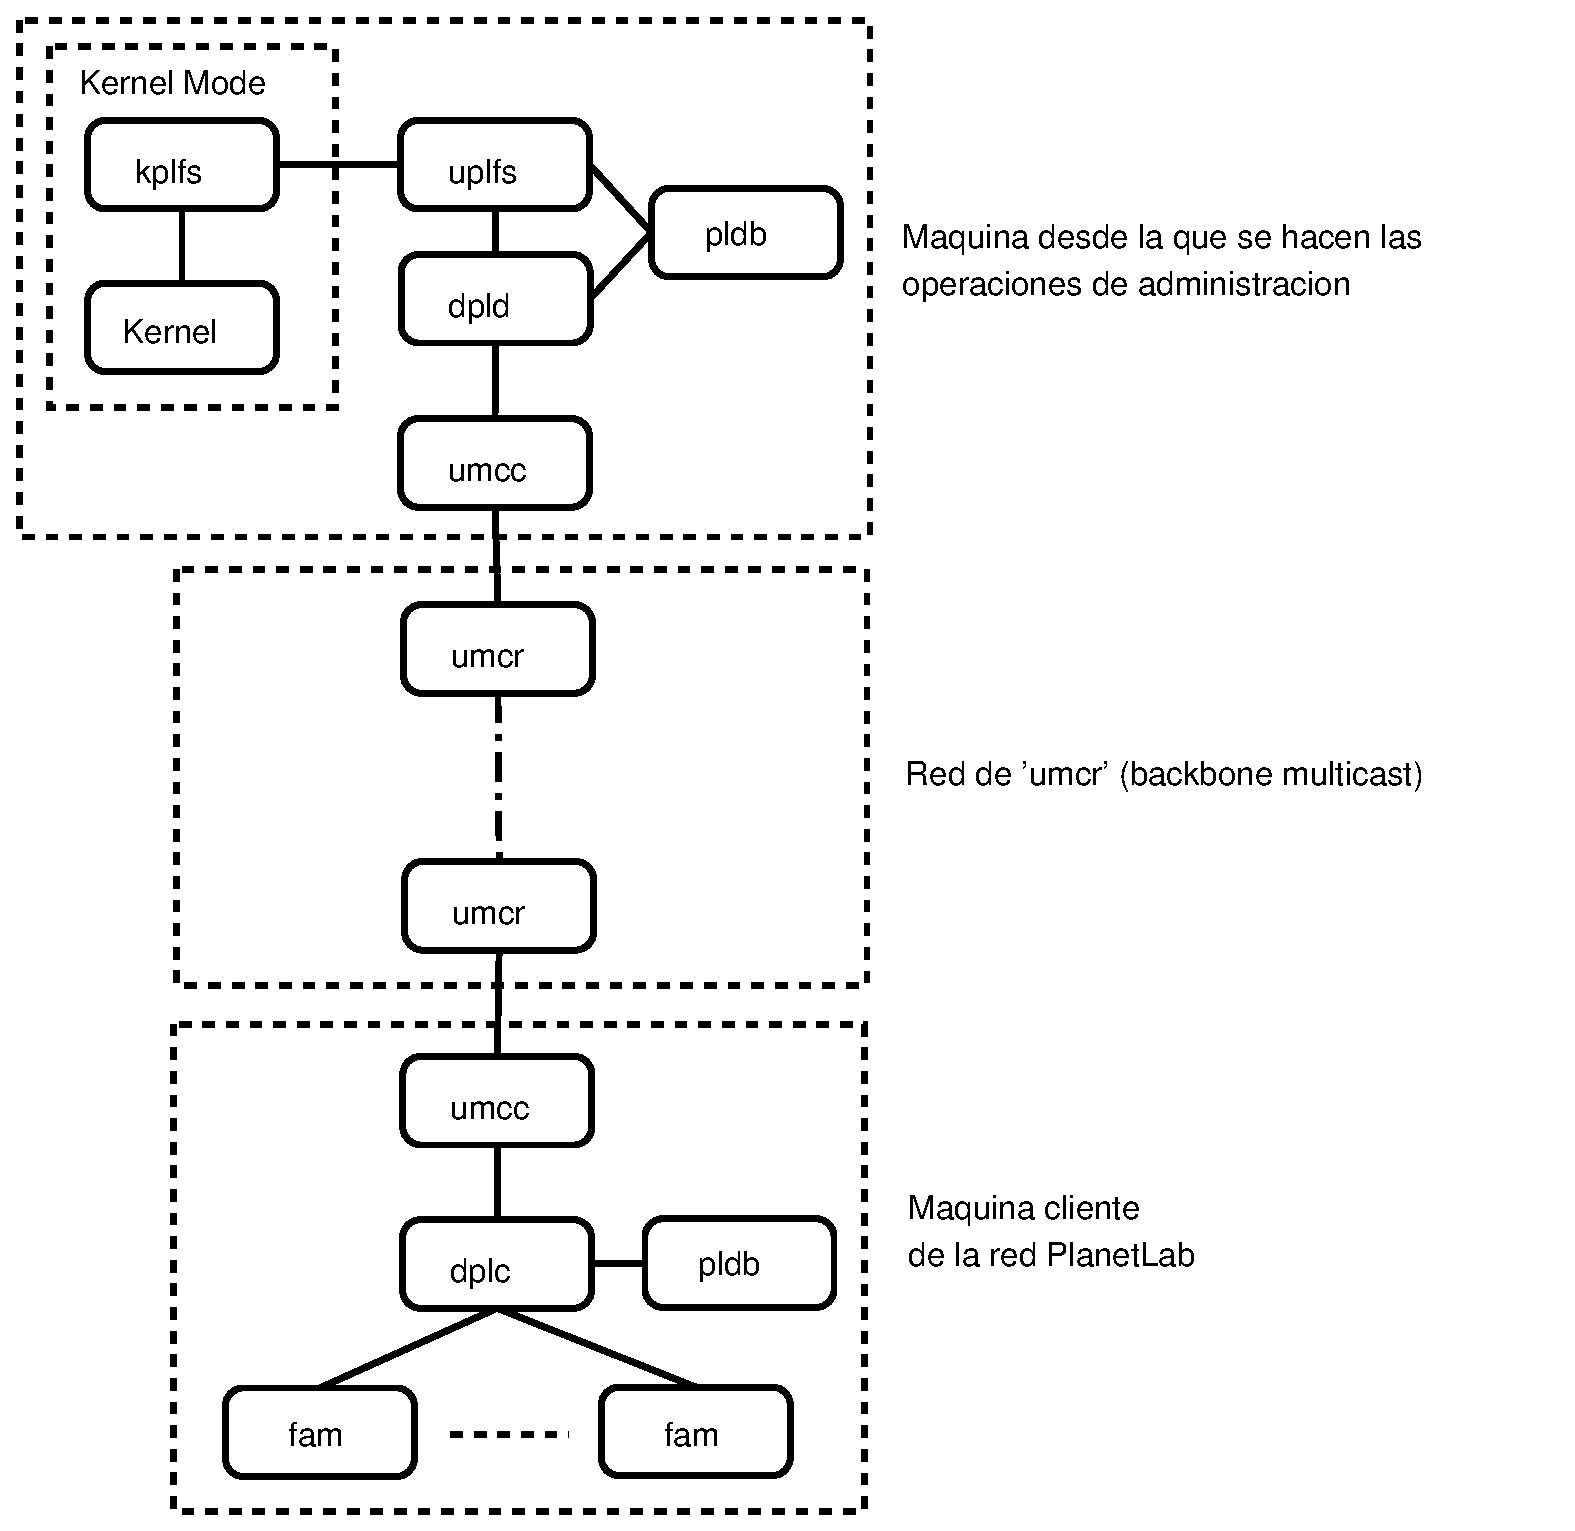
\includegraphics[scale=0.5]{arquitectura.eps}
	\caption{Arquitectura del Sistema}
	\label{fig:arquitectura}
\end{figure}



\section{L�gica del sistema}

\begin{itemize}
	\item Descubrimiento de slices en PlanetLab \\
		Al acceder al sistema de ficheros (\kplfs-\uplfs), hay que preguntar a
		un servicio de PlanetLab si existe o no un slice dado (al hacer un
		move de un ejectuable a un directorio que es un slice) o cu�les
		existen (al hacer un ls para ver los slices disponibles).

		Para ello, hace falta encontrar el nodo con el servicio de PlanetLab
		de BD \textbf{m�s cercano} (por ahora solo hay uno, y es
		\textit{PlanetLab Central}) y preguntarle:
		\begin{itemize}
			\item si existe un slice concreto

			\item qu� slices hay
		\end{itemize}

	\item Descubrimiento de nodos en PlanetLab \\
		Como en el caso anterior, nos hace falta preguntar a PlanetLab por los
		nodos, tanto a nivel general, como por los asociados a un slice.

	\item Descubrimiento del nodo de entrada a la red de distribuci�n
		multicast.
\end{itemize}

Con tal de minimizar la latencia y ocupaci�n innecesaria del ancho de banda,
para todos los anteriores puntos hace falta encontrar el nodo m�s cercano que
da un servicio concreto.

Para ello, se podr�a utilizar un servicio DNS al estilo Akamai, tal como
utiliza google, o algo como CoDNS \cite{CoDNS}, subproyecto de Codeen
\cite{Codeen}, que nos dan la IP del nodo m�s cercano que proporciona un
servicio conreto.



\section{Esquema de \plfs (PlanetLab File System)}

%\newpage
\begin{code}
	/plfs
	|-slices
	| `-<slice>
	|   |-key
	|   |-passwd
	|   |-script
	|   |-nodes
	|   | `-<node>
	|   |   `-unshared
	|   `-shared
	`-nodes
	  `-<node>
	    `-slices
	      `-<slice> -> /plfs/slices/<slice>
\end{code}

\begin{description}
	\item[\texttt{/plfs/slices/\textless{}slice\textgreater/key}] :\\
		�ste fichero contiene la clave privada ssh correspondiente al slice.

	\item[\texttt{/plfs/slices/\textless{}slice\textgreater/passwd}] :\\
		�ste fichero contiene el password asociado a la clave privada del
		slice.

	\item[\texttt{/plfs/slices/\textless{}slice\textgreater/script}] :\\
		�ste fichero es un shell script que se ejecutar� en cada m�quina una
		vez hecho el desplegamiento.
		\\
		El script tiene un s�lo par�metro que puede ser:

		% TODO(~): NOTA MENTAL: �al terminar la m�quina virtual, ya
		% ejecutar� dicho startup->stop?
		\begin{description}
			\item [start:] lleva a cabo las operaciones para
				arrancar el servicio desplegado

			\item [stop:] lleva a cabo las operaciones para parar
				el servicio

			\item [deploy:] lleva a cabo las operaciones necesarias
				para preparar el arranque del servicio
		\end{description}

	\item[\texttt{/plfs/slices/\textless{}slice\textgreater/nodes/\textless{}node\textgreater/unshared}] :\\
		�ste directorio es propio de cada nodo en el contexto del slice que
		estamos mirando; puede servir para guardar ficheros de configuraci�n
		espec�ficos de cada m�quina, sin hacer nunca un desplegamiento al
		grupo entero.

	\item[\texttt{/plfs/slices/\textless{}slice\textgreater/shared}] :\\
		�ste directorio contiene los ficheros de los que se hace un
		desplegamiento al grupo entero (slice). La condici�n que deben
		cumplir los contenidos de �ste directorio, es que sean
		inmutables de cara a \plfs.
\end{description}

Tal como est� hecho el esquema, permitir�a que alguien pusiera un directorio
de administraci�n en, por ejemplo,
\texttt{/plfs/slices/\textless{}slice\textgreater/monitor} con estad�sticas de
funcionamiento del slice, u otro
\texttt{/plfs/nodes/\textless{}node\textgreater/monitor} con estad�sticas de
funcionamiento de un nodo concreto.



\section{Operaciones de \plfs}

Las posibles operaciones que \plfs permite, y por ende, que \kplfs implemente
y puede llegar a comunicar a \uplfs, son las propias de un sistema de
ficheros, es decir (seg�n las operaciones que puede realizar un usuario desde
la l�nea de comandos):

\begin{description}
	\item [\texttt{ls}] :\\
		Operaciones de consulta de contenido de directorios y/o
		propiedades.

		\begin{itemize}
			\item Listado de slices (v�a m�dulo \pldb)

			\item Listado de nodos (v�a m�dulo \pldb)

			\item Listado de ficheros desplegados (\texttt{shared}
				y \texttt{unshared}).
		\end{itemize}

	\item [\texttt{mv}] :\\
		Lo que nosotros implementaremos ser� un \textit{move} de ficheros
		(aplicaci�n a desplegar) a un slice (conjunto de nodos, representado
		por el directorio
		\texttt{/plfs/slices/\textless{slice\textgreater/shared}}) o nodo
		concreto (representado por el directorio
		\texttt{/plfs/slices/\textless{slice\textgreater/nodes/\textless{}node\textgreater/unshared}}).
		Es decir, \textbf{no} permitiremos operaciones como:

		\begin{itemize}
			\item mover nodos

			\item mover slices

			\item \ldots
		\end{itemize}

	\item [\texttt{cp}] :\\
		Igual que en un \textit{move}, pero copiando los ficheros de or�gen.

	\item [\textit{edici�n}] :\\
		La edici�n de un fichero provocar� el redespliegue del mismo
		una vez sea cerrado.

	\item [\textit{lectura}] :\\
		La lectura de un fichero provocar� su importaci�n previa en
		caso de no estar cacheado.

	\item [\texttt{rename}] :\\
		Soportado solo para ficheros y directorios que cuelgan de
		\texttt{shared} o \texttt{unshared}.

	\item [\texttt{rm}] :\\
		Soportado solo para ficheros y directorios que cuelgan de
		\texttt{shared} o \texttt{unshared}.

	\item [\texttt{mkdir}] :\\
		Seg�n en que directorio se haga, las implicaciones son
		distintas:

		\begin{itemize}
			\item En \texttt{/plfs/slices}: Crea un slice sin nodos asociados

			\item En \texttt{/plfs/slices/\textless{}slice\textgreater/nodes}:
				A�ade un nodo a un slice

			\item En \texttt{/plfs/nodes}: A�ade un nodo al sistema
				PlanetLab

			\item En los directorios \texttt{shared} y
				\texttt{unshared} crea �se directorio, seg�n
				corresponda
		\end{itemize}

		Los tres primeros puntos, como no entran dentro del
		desplegamiento de aplicaciones, no han sido pensados en
		profundidad para llevarlos a cabo.

	\item [\texttt{rmdir}] :\\
		Igual que en el caso anterior, seg�n en que directorio se haga, las
		implicaciones son distintas:

		\begin{itemize}
			\item En \texttt{/plfs/slices}: Elimina un slice de PlanetLab

			\item En \texttt{/plfs/slices/\textless{}slice\textgreater/nodes}:
				Elimina un nodo de un slice

			\item En \texttt{/plfs/nodes}: Elimina un nodo del sistema
				PlanetLab

			\item En los directorios \texttt{shared} y
				\texttt{unshared} elimina el directorio que
				corresponda.
		\end{itemize}

		De nuevo, los tres primeros puntos, como no entran dentro del
		desplegamiento de aplicaciones, no han sido pensados en
		profundidad para llevarlos a cabo.

	\item [\texttt{touch}] :\\
		\textbf{NO} soportado.

	\item[\texttt{chown}, \texttt{chmod}] :\\
		\textbf{NO} soportado.

	\item[\texttt{ln}] :\\
		\textbf{NO} soportado.

	\item[Otras operaciones] :\\
		\textbf{NO} soportadas.
\end{description}



\section{L�gica de Desplegamiento}

Cada vez que se realiza un move/copy en el sistema de ficheros para el
desplegamiento, los pasos a seguir son estos:

\textit{Precondici�n}: El slice destino est� ya creado (\texttt{mkdir}).

\begin{enumerate}
	\item \kplfs $\rightarrow$ \uplfs \\
		Se informa de los ficheros de aplicaci�n a desplegar i del slice
		o nodo destino (en el caso de ser un solo nodo el
		destino, la comunicaci� se establece directamente
		desde \uplfs hacia \dplc).

	\item \uplfs $\rightarrow$ \dpld \\
		\uplfs redirige el mensaje al componente indicado por este (\dpld),
		puesto que \kplfs puede manejar la vista de diferentes componentes.

	\item \dpld $\rightarrow$ \umcc \\
		Se comunica el slice destino, se dan los ficheros a desplegar y el
		shell script con los comandos a ejecutar una vez desplegados.

	\item \umcc $\rightarrow$ red \umcr \\
		Se inyectan los paquetes a enviar con destino a un grupo en la
		red \umc.\\
		En nuestro caso, el grupo destino ser�a un slice y el
		desplegamiento se realizar� a aquellos nodos donde haya \dplc,
		de modo que ser�n siempre conocidos por la red multicast.

	\item intra-red \umcr (red multicast) \\
		Los nodos de la red \umcr encaminan el conjunto de paquetes
		hacia el grupo multicast de destino.\\
		En nuestro caso encaminar�n los ficheros, script, etc de
		la aplicaci�n a desplegar hacia los nodos de \dplc que forman
		parte del slice destino.

	\item red \umcr $\rightarrow$ \umcc \\
		Los paquetes llegan finalmente a los nodos que conforman el
		grupo destino multicast.
		En nuestro caso, los ficheros, script, etc. llegan finalmente a
		los nodos destino y son procesados por el m�dulo \umcc.

	\item \umcc $\rightarrow$ \dplc \\
		El m�dulo \umcc hace llegar los paquetes a desplegar al \dplc.

	\item \dplc $\rightarrow$ slice destino (ssh) \\
		Se despliega la aplicaci�n (se copian los ficheros), y una vez hecho
		esto, se ejecuta el shell script adjuntado, en caso de estar
		presente. Para ello, primero ejecuta el \textbf{deploy} y luego
		el \textbf{start}.
		En el apartado de sincronizaci�n veremos con m�s detalle las
		diferentes posibilidades al realizar la ejecuci�n del script
		(sincronizaci�n).
		%TODO: CITE => cite de que?!
\end{enumerate}

% TODO: NOTA:
% En caso de haber un fallo en cualquiera de los dos pasos anteriores,
% se devuelve un error al dpld origen (a modo de NACK) ??????
% Si todo es correcto anunciar al dpld??? Escalabilidad? ACK's



\section{Comunicaci�n Multicast}

Como hemos comentado, el desplegamiento de los ficheros se hace sobre una red
multicast, por lo que hace falta describir algunas de sus caracter�sticas que
asumiremos de ahora en adelante para el dise�o de los componentes del sistema.

Las operaciones que debe proporcionar esta red multicast son las siguientes:

\begin{description}
	\item[Join]:\\
		Inscripci�n a un grupo multicast.

	\item[Leave]:\\
		Desuscripci�n de un grupo multicast.
\end{description}

En nuestro caso, veremos como \dplc gestiona las inscripciones/desuscripciones
a los grupos multicast, dichos grupos ser�n realmente los slice destino a los
que se quiera realizar el desplegamiento de las aplicaciones. De modo que,
cuando se quiera hacer dicho desplegamiento, desde \dpld, no ser� necesario
consultar previamente a PlanetLab Central (mediante \pldb) sobre la pertinencia
de los nodos a un grupo. Es decir, el grupo ya est� previamente creado.

El modo en que \dplc realiza las operaciones de inscripci�n/desuscripci�n y en
qu� momento, lo veremos con m�s detalle en el cap�tulo \ref{TODO}.
%TODO CITE

Para hacer que la red multicast sea fiable nos hemos planteado las siguientes
posibilidades:

\begin{description}
	\item[NACK based]:\\
		Solamente se env�an NACKS en caso de fallo en el env�o. Es
		decir, no se realizan ACK's.

	\item[Tree ACK (TRACK)]:\\
		En este caso, se env�an ACK's pero agrupados hacia la ra�z del
		�rbol multicast. Es decir, los ACK's de los "hijos" se agrupan
		en el "padre" para enviar un s�lo ACK.
\end{description}

En nuestro caso, hemos pensado que ser�a positivo elegir la opci�n de TRACK,
puesto que �sta nos permitir�a que \dpld realizara los tipos de
desplegamiento que presentamos en el apartado \ref{sect-deployment}.
%TODO CITE



\section{Tipos de Desplegamiento}
\label{sect-deployment}

Los tipos de desplegamiento que hemos considerado interesantes son los
siguientes:

\begin{description}
	\item[Desplegamiento immediato]:\\
		Una vez desplegados los ficheros, se ejecuta el script de
		desplegamiento y arranque.

	\item[Desplegamiento sincronizado]:\\
		Gracias a la implementaci�n TRACK de Multicast, podemos hacer
		un desplegamiento sincronizado a dos pasos, en primer lugar
		realizamos el desplegamiento de los ficheros, y una vez recibido
		el ACK agrupado realizamos una segunda comunicaci�n multicast
		para ejecutar el script de desplegamiento y arranque.

	\item[Redesplegamiento]:\\
		Se realiza de la misma manera que un desplegamiento immediato,
		pero como reacci�n a una suscripci�n de un nuevo nodo, o bien
		al reintento de desplegamiento en un nodo en el que ha fallado
		un desplegamiento previo (NACK).

		% TODO ESPECIFICAR COMO ELEGIR EL TIPO DE DESPLEGAMIENTO

		% TODO(~) (Apartats3.2, 3.6 i 4.3):
		%
		%	A�adir un nodo al slice una vez ya desplegada la
		%aplicacion
		%
		%	Solucio: DPLC d'aquest node, ha de comunicar a DPLD que
		%	s'hi afegeix al qual se li ha de fer desplegament!! (3.2, 3.6)
		%		=> PROTOCOL DE WARNINGS AMB AUTENTIFICACIO!!! (4.1)
		%
\end{description}


% TODO (!!!!!): Cuando se abren las conexiones SSH? timeout?
%       Cuando se dan las claves y passwd ssh?
%


% TODO(?): 'ls' => renew => cheksums??
%
% TODO(~)  'ls' de unshared ??
% 	=> MIRAR NODO CONCRETO => DPLC TIENE QUE AGREGAR FUNCIONALIDAD 	(3.6)
%
% TODO(~)  'ls' de shared ??
%
%	Solucio Possible:
%		1) dpld escull a l'atzar un node del slice a qui preguntar
%		<shared> (essent aquest no corrupte).			(3.2)
%		2) si dpld s'assabenta que un node es corrupte, envia l'ordre
%		de fer stop.
%			a) si no es sincrhonized, el redesplega amb
%			deployAppToNode
%			b) si es synchronized,
%				- Redesplegar tot per ex. si hi ha un minim de
%				nodes no corruptes i en funcionament.
%
%
%	=> FAM ha de comunicar a DPLC si hi ha canvis als fitxers
%		=> FAM ha de saber quins fitxers son shared		(3.7)
%		=> DPLC ha d'arrancar FAM!!!				(3.6)
%
%	A MES SI FAM SAP SI SON SHARED O UNSHARED, permet que DPLC li soliciti
%	els fitxers de cada tipus segons la peticio que faci DPLD.


\chapter{Dise�o de los componentes}

\textbf{\textit{En este cap�tulo definimos las principales funcionalidades que
deben implementar cada uno de los componentes.}}



\section{\kplfs}
Este m�dulo implementa la interfaz del VFS, y las operaciones que permite las
hemos descrito en el cap�tulo anterior en el apartado de L�gica de
Desplegamiento 2.5.

% TODO(?): invalidate



\section{\uplfs}

Las operaciones que \uplfs ofrece, adem�s de las especificadas en el m�dulo
\pldb para las que hace de intermediario, son las siguientes:

%TODO: es solo esto?
\begin{description}
	\item[\texttt{execute(component, operation, \ldots)}] :\\
		Llama a la funci�n \texttt{operation} del componente
		\texttt{component} con los par�metros extra que se indiquen (en caso
		de indicar alguno).
\end{description}



\section{\dpld}

Las operaciones que \dpld ofrece son las siguientes:

% TODO: faltan las credenciales de autentificacion, o mejor un paso previo de
% autentificaci�n?!?!?!?!
% TODO(~): faltan los parametros de que desplegar, etc
% TODO(~): explicar fichero de comandos etc otra vez? 		NOO!!
% TODO(~): poner los resultados de las ops
\begin{description}
	\item[\texttt{void deployAppToSlice (slice\_name, files[], script, key,
		passwd,...)}] :\\
		Realiza la comunicaci�n con el componente \umcc para desplegar
		una aplicaci�n (files) a trav�s de la red \umcr en el grupo
		indicado por el slice\_name. Para ello tambi�n requerir� el
		script de inicializaci�n, y la clave y password de ssh del
		slice.
		\\
		% TODO: pero ahora hay TRACK!!!
		% primer intento + reintentos a solo a quien falla? (pero por multicast si cierto numero)
		NOTA: La operaci�n no puede devolver resultado de �xito,
		puesto que la implementaci�n de ACKS en Multicast tiene
		problemas de escalabilidad, y por lo que hace a los NACKS
		no creemos que sea muy bueno mantener el \dpld esperando a ver
		si recibe alguno.

	\item[\texttt{ void deployAppToNode (slice\_name,
		node\_name,files,script, key, passwd) }] : \\
		Lo mismo que deployAppToSlice pero hacia un nodo concreto.
		�til, si se a�ade un nodo a un slice al que se ha realizado ya
		el desplegamiento.

	\item[\texttt{void addNodeToSlice (slice\_name, node\_name)}] :\\
		Crea el directorio que representa al nodo en el sistema de
		ficheros y posteriormente ejecuta \texttt{deployAppToNode}.

	\item[\texttt{registerToDplc (node\_name, slice\_name)}] :\\
		Se registra el nodo de \dpld como oyente de los cambios que se
		producen en un slice de un nodo concreto.
		% TODO(?): se puede utilizar un grupo de oyentes a cambios en
		% grupos de dplc, asi no hace falta el registro...

	\item[\texttt{invalidateObj (slice\_name, name)}] :\\
		% TODO(?): utilizar identificador de obj diferente del path?
		% hace falta nombre del slice? (path completo)
		Invalida un objeto del sistema de ficheros (un fichero o un
		directorio).
		%NOTA: de que puede servir invalidar un objeto del FS?

	% TODO(?): validaciones? temporalidad?     ES UTIL PLANTEARSELO?
	
	% TODO: quien lo utiliza?
	\item[\texttt{getInfoFilesShared (slice\_name)}] :\\
		Env�a una petici�n a multicast de informaci�n de los ficheros
		de tipo \textit{shared} del slice \textit{slice\_name}.

	% TODO: quien lo utiliza?
	\item[\texttt{getInfoFilesUnshared (node\_name,slice\_name)}] :\\
		Env�a una petici�n unicast hacia el \dplc del nodo
		\textit{node\_name} de informaci�n acerca de los ficheros de
		tipo \textit{unshared} del slice \textit{slice\_name} para dicho
		nodo.
\end{description}



\section{\pldb}

\pldb permite acceder a informaci�n relativa a la administraci�n de slices y
nodos de PlanetLab.

En concreto, las operaciones que ofrece (API), son:

\begin{description}
	\item[\texttt{getSlices}] :\\
		Permite obtener la lista de slices que se han dado de alta en PlanetLab

	\item[\texttt{getNodes}] :\\
		Permite obtener la lista de nodos que se han dado de alta en PlanetLab

	\item[\texttt{getSlice (slice\_name)}] :\\
		Permite obtener informaci�n de un slice

	\item[\texttt{getNode (node\_name)}] :\\
		Permite obtener informaci�n de un nodo

	\item[\texttt{getSliceNodes (slice\_name)}] :\\
		Permite obtener los nodos que hay en un slice

	\item[\texttt{getNodeSlices (node\_name)}] :\\
		Permite obtener los slices de un nodo

	\item[\texttt{getSliceNode (slice\_name, node\_name)}] :\\
		Permite obtener informaci�n de un nodo de un slice

	\item[\texttt{getNodeSlice (node\_name, slice\_name)}] :\\
		Permite obtener informaci�n de un slice de un nodo

	\item[\texttt{addSlice (slice\_name)}] :\\
		Permite a�adir un slice

	\item[\texttt{addNode (node\_name)}] :\\
		Permite a�adir un nodo

	\item[\texttt{addSliceNode (slice\_name, node\_name)}] :\\
		Permite a�adir un nodo en un slice

	\item[\texttt{removeSlice (slice\_name)}] :\\
		Permite eliminar un slice

	\item[\texttt{removeNode (node\_name)}] :\\
		Permite eliminar un nodo

	\item[\texttt{removeSliceNode (slice\_name, node\_name)}] :\\
		Permite eliminar un nodo de un slice
\end{description}

Para obtener toda esta informaci�n, hace falta utilizar la API que ofrece
PlanetLab Central \cite{PLC}.



\section{\umcc}
\label{sect:umcc}

�ste es el m�dulo cliente de la red multicast, b�sicamente tiene dos
funciones:

\begin{description}
	\item Enviar los datos a desplegar al nodo \umcr m�s cercano.

	\item Recibir los datos a desplegar y hacerlos llegar al m�dulo dplc.
\end{description}

El primer caso, se da cuando \dpld ordena el desplegamiento de una
aplicaci�n/servicio hacia un slice destino. En este caso deber� comunicarse
con el m�dulo umcr m�s cercano para comunicarle los datos necesarios.
El segundo caso, se da cuando un nodo \umcr le comunica que se debe desplegar
una aplicaci�n/servicio en el nodo d�nde \umcc reside, en este caso deber�
comunicare con el m�dulo \dplc para hacerle llegar los datos de desplegamiento.

De modo que las operaciones que ofrece, son:

% TODO(~): seguridad a la hora de hacer cambios? umcc va en la m�quina de
% administracion (se puede modificar lo que se quiera)      .... I????
%TODO(?): ``dns''?  ------- PQ EL GRUPID NO POT SER SLICE_NAME?
%			    TB SERVIRIA SI VOLEM ENVIAR A SLICE
%			    DPLD WARNINGS
\begin{description}
	\item[\texttt{group\_id getGroup (group\_name)}] :\\
		Permite obtener el identificador, dentro de la red \umc, de un grupo.

	\item[\texttt{setOptions (group\_id, options[])}] :\\
		%TODO(?): QUE FA AIXO??
		%TODO(?): necesario? depende del soft multicast de debajo

	\item[\texttt{sendData (group\_id, data)}] :\\
		Permite enviar datos a un grupo

	\item[\texttt{recieveData (group\_id, data)}] :\\
		Recibe datos procedentes de un emisor del grupo, y se los pasa
		al m�dulo \dplc (quien se encargar� del despliegue.

	%TODO(~): addGroup / deleteGroup ?

	\item[\texttt{join (group\_name, node\_name)}] :\\
		%TODO(?): hace falta el nombre o ya va bien por remitente?
		%TODO(?): c�mo hacer el join de otro?
		Permite a�adir un nodo a un grupo multicast

	\item[\texttt{delete (group\_id, node\_name)}] :\\
		%TODO(?): hace falta el nombre o ya va bien por remitente?
		%TODO(?): c�mo hacer el delete de otro?
		Permite eliminar un nodo de un grupo multicast
\end{description}

La ventaja de �ste m�dulo es que es totalmente inocuo, por lo que se puede
utilizar la arquitectura de \umc (\umcc + \umcr) en cualquier aplicaci�n, y
permite que se puedan utilizar otros proyectos ya realizados.

% TODO(~): estudiarlo!!!
% El punto que a�n no hemos aclarado es si el propio identificador de grupo
% multicast ser� el identificador de slice (VOTO POR ELLO!!!!!!!!!!!) o algun
% otro de m�s gen�rico (que requerir�a una nueva capa de administraci�n de
% grupos multicast).
%
% Depende del software de multicast que se utilize! (araneola)



\section{\umcr}

Estos nodos se encargan de hacer la transimisi�n multicast, con tal de hacer
llegar los datos a los \umcc del grupo de destino.
Asumiremos que estos nodos pertencen a un slice administrativo en el cual no se
realizan modificaciones o configuraciones maliciosas.

C�mo todos los accesos a la red multicast se hacen a traves de \umcc, se puede
f�cilmente utilizar una implementaci�n ya existente de una red overlay
multicast en modo usuario, como es Araneola \cite{Araneola}.

%TODO(!!!): EXPLICAR ARANEAOLA SI ES LA UNICA SOLUCIO
%TODO: Operaciones?



\section{\dplc}

% TODO: pertenece a un slice administrado correctamente (no habra
% modificaciones ni configuraciones maliciosas)

�ste m�dulo, situado en cada una de las m�quinas clientes (o receptoras de las
aplicaciones de las que queremos hacer el desplegamiento), se sit�a en un
slice propio (donde estar�n todos los nodos con �ste m�dulo), y al recibir los
datos de \umcc acceder� a s� mismo por ssh con tal de poner los ficheros al
slice destino y seguidamente ejecutar el shell script asociado, en caso de
estar presente.

Para realizar esta conexi�n por ssh, el nodo del slice dplc necesita los datos
de clave y password ssh para que \dplc pueda hacer una conexi�n a la propia
m�quina y acceder a la m�quina virtual asociada al slice de destino.

Para ello, se podr�a pensar en varias soluciones, como son:

\begin{description}
	\item Realizar una preautentificaci�n, en la que dplc se autentifica con los
		slices a los que se llevar� acabo el deployment de aplicaciones, de modo que en
		las comunicaciones no haga falta realizar el env�o de clave y password y tampoco
		tener que preocuparse de como hacerlo de forma segura.

	\item Que en cada comunicaci�n se env�en, adem�s de los ficheros, los datos de
		autentificaci�n (clave ssh y password).

		% TODO(~): pre-autentificacion? JUSTIFICAR PERQUE HEM FET LA SEGONA :-S
\end{description}

De modo que las operaciones que debe implementar este m�dulo son las
siguientes:

% TODO(?): seguridad?
\begin{description}
	% TODO: que es _la informacion_?
	\item[\texttt{getInfoNodeSlice(slice\_name)}] :\\
		Obtiene la informaci�n de los ficheros tipo \textit{unshared}
		de la aplicaci�n desplegada en el slice \textit{slice\_name} en
		el mismo nodo que el propio \dplc.

	% TODO: ELIMINAR: llama a la operacion, no la ofrece
	\item[\texttt{warnDpldNewNodeInSlice (slice\_name, node\_name)}] :\\
		Avisa a los \dpld encargados del slice \textit{slice\_name} de
		que se ha agregado un nuevo nodo \textit{node\_name} a dicho a
		slice y que por lo tanto se le deber�a realziar el despliegue de
		la aplicaci�n.

	\item[\texttt{deployAppToSlice (slice\_name, ...)}] :\\
		Realiza la conexi�n por ssh al slice destino, despliega la
		aplicaci�n y ejecuta el script de inicializaci�n.

	\item[\texttt{registerToDplc (node\_name, slice\_name)}] :\\
		Un nodo se registra en \dplc como integrante del slice
		slice\_name al que se va realizar desplegamiento de
		aplicaciones.

	% TODO: para que? se para sola... hace falta ofrecer la opcion de pararla?
	\item[\texttt{stopAppInSlice (slice\_name)}] :
		El \dplc del nodo ejecutar� script->stop en el slice
		\textit{slice\_name} de dicho nodo. Es decir, detendr� la
		aplicaci�n desplegada en �l.

	\item[\texttt{invalidateObj (slice\_name, name)}] :\\
		% TODO(~): utilizar identificador de obj diferente del path?
		% hace falta nombre del slice? (path completo) <<-- PATH COMPLET
		Invalida un objeto del sistema de ficheros (un fichero o un
		directorio)

	% TODO(?): validaciones? temporalidad?
\end{description}

% TODO(~): se�alar los triggers de join / delete de los grupos

% TODO:
%Cuando se a�ade un nodo a un slice en el que se realiza desplegamiento, se
%tiene que informar al m�dulo \dpld, puesto que es posible que ya se hubiera
%realizado un desplagamiento previo a dicho slice y \dpld tenga que realizar un
%deployment al nodo en concreto.
%
%Para ello hemos pensado en un protocolo de "warnings" en el que \dplc realizara
%comunicaciones multicast hacia los nodos \dpld, comunic�ndoles:
%	- nodo
%	- slice
%
% ===>>> LA QUAL COSA ACABARIA AMB L'OPERACIO QUE HE AFEGIT addNodeToSlice de
%	dpld
%
% Como diferenciar al entrar un nodo en un grupo de si ya esta al dia o no?
% - no se hace nada (solo hay cambios si esta presente en un deploy expreso)
% - tiene la ultima version de los ficheros (numeracion + indicador de ultima version (*))
% - los tiene igual que la mayoria (checksums + problema bizantino)
% - los tiene igual que un repositorio (checksums + repositorio - bamboo? -)
%
% (*) Puede ser:
% o el nunmero mas grande que den los miembros del grupo
%   - deben responder todos
%   - alguien puede enga�arnos y dar un numero equivocado?
%   -> dplc nos firma la version -> garantiza la validez (como el algodon, 
%     dplc nuca enga�a)
% o el numero que den la mayoria
%   - deben responder todos
%   - podemos tirar a una version anterior (pq la mayoria de ahora no estaban
%     presentes en un deployment anterior y decidieron al connectar que la
%     version era esta)
% o lo que digan los dpld (mayoria o maximo)
%   - debe haber dpld en marcha
%   + #dpld < #dplc
% o lo que diga un repositorio central
%   - poca escalabilidad
%   - punto unico de fallada
%   + resultados fiables
%
% Al detectar un desfase de las versiones (nodo corrupto?), que hacer:
% - protocolo de las transparencias
% - parar y esperar al siguiente deployment



\section{\famon}

�ste m�dulo est� situado en las m�quinas clientes de la red, y se encarga de
monitorizar los ficheros que han sido desplegados en un nodo de un slice.

Para ello debe haber una instancia corriendo en cada m�quina virtual que
corresponda a un slice que funciona a traves de \plfs.

% TODO: quien/cuando se arranca?
% TODO: que se vilgila?
% - ficheros desplegados expresamente
% - ficheros resultado de (genereados despues de) desplegar y/o arrancar la aplicacion
%   (como se detecta que crea la aplicacion y que lo hace el usuario u otro proceso que no es
%   la aplicacion desplegada?)
%   (si se detecta, como diferenciar shared/unshared?)
%
% Yo solo vigilaria lo desplegado expresamente.

% TODO (no va aqui)
% script->deploy : depliega la aplicacion y guarda una lista de ficheros extra generados en la posible descompresion
%    (mejor script->install)
% script->remove : elimina los ficheros instalados, para poder instalar otra vez (posible nueva version)
% script->update?

% Las operaciones que debe ofrecer \famon son las siguientes:
% TODO: operaciones de viliar / dejar paths concretos?

% TODO: buscar un buen programa que lo haga => famd, gamin?

\chapter{Comunicaci�n entre los componentes}

\textbf{\textit{En este cap�tulo comentamos diferentes implementaciones de la
comunicaci�n entre componentes del sistema. Como veremos, nos centraremos en
los tipos de mensajes en cada tipo de comunicaci�n y la seguridad que debemos
implementar en cada una, para asegurar autenticidad y confidencialidad.}}
\\

Las comunicaciones entre componentes de un mismo nodo funcionan a modo de
llamadas ``normales'' entre partes de un mismo programa (aunque se carguen en
forma de \textit{plugins}).

La comunicaci�n entre componentes de nodos separados se realiza siempre mediante
el paso de mensajes que siguen �ste formato:

\begin{enumerate}
	\item IDoperaci�n

	\item Remitente

	\item Datos de la operaci�n (par�metros o resultado)
\end{enumerate}

Seguidamente pasamos a concretar los detalles de comunicaci�n de los diferentes
componentes.



\section{\kplfs $\longleftrightarrow$ \uplfs}

Para que la aplicaci�n en modo usuario pueda enterarse de las operaciones
que se realizan sobre el sistema de ficheros, el m�dulo \kplfs a nivel de
kernel, debe comunicarse con el m�dulo \uplfs a nivel usuario.
Para realizar esta comunicaci�n de eventos, hay varias posibilidades:

\begin{description}
	\item [Dispositivo:]
		Aprovecha las propias caracter�sticas de un dispositivo de
		sistema, ya que permite hacer esperas no activas (es decir
		bloqueantes), a trav�s de \textit{poll}, \textit{read},
		\textit{select} de un dispositivo que implementa \kplfs.

	\item [Compartici�n de memoria:]
		El problema de esta soluci�n es que requiere una espera activa
		por parte de \uplfs, que debe ir comprobando la zona de memoria
		compartida para ver si hay alg�n nuevo evento procedente de
		\kplfs.
\end{description}

As� pues, por las ventajas de operaciones no bloqueantes que ofrece,
utilizaremos un \textbf{dispositivo} para comunicar ambos componentes.

Cuando se realice una operaci�n (\texttt{ls},\texttt{mv}, etc) en el sistema
de ficheros \plfs, el m�dulo de kernel \kplfs que implementa estas operaciones,
deber� informar dichos eventos al m�dulo a nivel usuario \uplfs (el cual deber�
realizar las operaciones pertinentes, comunic�ndose con los diferentes
componentes disponibles y respondiendo a cada operaci�n con su identificador
\texttt{id}).

En �ste caso, aunque los componentes est�n en el mismo nodo, deben enviarse
mensajes a trav�s del dispositivo de control, mensajes que tienen el mismo
formato que se ha comentado al inicio del cap�tulo, pero sin el par�metro de
\texttt{Remitente}.
\\

\kplfs $\rightarrow$ \uplfs:

\begin{itemize}
	\item \texttt{execute (component, id, operation, \ldots)}
\end{itemize}

\kplfs $\leftarrow$ \uplfs:

\begin{itemize}
	\item Operaciones para el retorno del resultado de las peticiones del
		VFS a \uplfs (ver \cite{lkapi}).
	\item \texttt{invalidate (slice\_name, node\_name, type, path)}
\end{itemize}



\section{\uplfs/\dpld/\dplc $\rightarrow$ \pldb}

Llamada interna de funciones.
\\

\uplfs/\dpld/\dplc $\rightarrow$ \pldb:

\begin{itemize}
	\item \texttt{getSlices ()}
	\item \texttt{getNodes ()}
	\item \texttt{getSliceNodes (slice\_name)}
	\item \texttt{getSliceNodesAny (slice\_name, num)}
	\item \texttt{getSliceNodesNumber (slice\_name)}
	\item \texttt{getSliceNode (slice\_name, node\_name)}
	\item \texttt{getSliceNodeAny (slice\_name)}
	\item \texttt{getSliceNodeNearest (slice\_name)}
	\item \texttt{getNodeSlices (node\_name)}
\end{itemize}



\section{\uplfs $\longleftrightarrow$ \dpld}

Llamada interna de funciones.
\\

\uplfs $\rightarrow$ \dpld:

\begin{itemize}
	\item \texttt{deployToSlice (slice\_name, path\_from, path\_to)}
	\item \texttt{deployToNode (slice\_name, node\_name, path\_from,
		path\_to)}
	\item \texttt{getInfoShared (slice\_name, path)}
	\item \texttt{getInfoUnshared (slice\_name, node\_name, path)}
	\item \texttt{getFileShared (slice\_name, path)}
	\item \texttt{getFileUnshared (slice\_name, node\_name, path)}
	\item \texttt{deleteFileShared (slice\_name, path)}
	\item \texttt{deleteFileUnshared (slice\_name, node\_name, path)}
	\item \texttt{getSliceNodeVersion (slice\_name, node\_name)}
	\item \texttt{registerNeeded (slice\_name, node\_name)}
\end{itemize}

\uplfs $\leftarrow$ \dpld:

\begin{itemize}
	\item \texttt{invalidate (slice\_name, node\_name, type, path)}
\end{itemize}



\section{\dpld $\longleftrightarrow$ \dplc}
\label{sect:warnings}

Teniendo en cuanta que cada componente tiene su propio par de llaves
(un par $K_{pub_{d}}$ y $K_{priv_{d}}$ para cada \dpld y un mismo par
$K_{pub_{c}}$ y $K_{priv_{c}}$ para todos los \dplc), todas las comunicaciones
van cifradas con la clave p�blica del emisor (para asegurar que s�lo
los receptores puedan leer los contenidos) y firmadas con la clave
privada del emisor (para poder as� comprobar su autenticidad), excepto
\texttt{getKey}, que s�lo va firmada.

Luego, en el destino, se comprueba la firma, se descifran los datos y se
procede a realizar la operaci�n pertinente.
\\

\dpld $\rightarrow$ \dplc:

\begin{itemize}
	\item \texttt{deployToSlice (slice\_name, path\_to, file, type,
		new\_version)}
	\item \texttt{getInfo (slice\_name, path)}
	\item \texttt{getFile (slice\_name, path)}
	\item \texttt{deleteFile (slice\_name, path, new\_version)}
	\item \texttt{getVersion (slice\_name)}
	\item \texttt{getKey ($K_{pub_{d}}$)}
	\item \texttt{registerWithResponse (slice\_name, $K_{SSH}$, $P_{SSH}$,
		$K_{pub}$)}
	\item \texttt{register (slice\_name, $K_{SSH}$, $P_{SSH}$, $K_{pub}$)}
\end{itemize}

\dpld $\leftarrow$ \dplc:

\begin{itemize}
	\item \texttt{registerNeeded (slice\_name, node\_name)}
	\item \texttt{invalidate (slice\_name, node\_name, type, path)}
\end{itemize}



\section{\dplc $\rightarrow$ \dplc}

Como la red de \dplc intenta llegar sola a la coherencia de versiones, necesita
ofrecer m�todos para ponerse en contacto e intercambiar datos, cifrando y
firmando con $K_{priv_{c}}$.

\begin{itemize}
	\item \texttt{deployToSlice (slice\_name, path\_to, file, type,
		new\_version)}
	\item \texttt{needDeploy (slice\_name, node\_name, path)}
	\item \texttt{ping (slice\_name, node\_name, version)}
	\item \texttt{getSSH (slice\_name)}
\end{itemize}



\section{\dpld/\dplc $\longleftrightarrow$ \umcc}

Llamada interna de funciones.

Cuando tanto \dpld como \dplc quieren comunicarse con un grupo (\dpld se
comunica con el grupo de receptores del slice para mandarles operaciones y
\dplc se comunica con el grupo de emisores para mandarles avisos), lo hacen a
trav�s de la red multicast, mediante el componente de entrada a ella que es
\umcc, de forma que mandan los datos como si fueran directamente como la
comunicaci�n anterior y se transmiten transparentemente por la red \umc.
\\

\dpld/\dplc $\rightarrow$ \umcc:

\begin{itemize}
	\item \texttt{group\_id getGroup (group\_name)}
	\item \texttt{setOptions (group\_id, options[])}
	\item \texttt{getOptions (group\_id, options[])}
	\item \texttt{sendData (group\_id, data)}
	\item \texttt{recieveData (group\_id, data)}
	\item \texttt{joinSender (group\_id, node\_name)}
	\item \texttt{deleteSender (group\_id, node\_name)}
	\item \texttt{joinReceiver (group\_id, node\_name)}
	\item \texttt{deleteReceiver (group\_id, node\_name)}
\end{itemize}

Con tal de saber \dpld cu�l es el estado de los slices, como la red multicast
subyacente puede informar de la adici�n y eliminaci�n de receptores, es el
propio \umcc quien se encarga de avisar a \dpld (en lugar de \dplc, evitando as�
ocupar la red innecesariamente).
\\

\dpld $\leftarrow$ \umcc:

\begin{itemize}
	\item \texttt{addNodeToSlice (slice\_name, node\_name)}
	\item \texttt{removeNodeFromSlice (slice\_name, node\_name)}
\end{itemize}

\dplc $\leftarrow$ \umcc son:

\begin{itemize}
	\item \texttt{joined (slice\_name)}
	\item \texttt{deleted (slice\_name)}
\end{itemize}



\section{\dplc $\longleftrightarrow$ \famon}

Llamada interna de funciones.
\\

\dplc $\rightarrow$ \famon:

\begin{itemize}
	\item \texttt{watch (path)}
	\item \texttt{unwatch (path)}
	\item \texttt{stop ()}
\end{itemize}

\dplc $\leftarrow$ \famon:

\begin{itemize}
	\item \texttt{invalidate (slice\_name, path)}
\end{itemize}

\chapter{Caminos de operaci�n}

\textbf{\textit{En este cap�tulo comentaremos los diagramas de secuencia que
seguir�an las comunicaciones entre los componentes para tener una idea general
del sistema de modo visual.}}



\section{Autentificaci�n}

Para la autentificaci�n con \dplc y verificaci�n de los datos firmados de �ste,
hace falta previamente conocer su clave p�blica.
%TODO: que pasa al recibir datos firmados/encriptados con una clave que no
%conocemos?

Con tal de acceder un cliente (\dpld) a un nodo (\dplc), �ste debe primero
registrarse envi�ndole la clave y password de SSH \textbf{encriptados} con la
clave p�blica de \dplc (para evitar que informaci�n sensible sea capturada).

Para ello, hay dos primitivas de autentificaci�n, una que hace una
autentificaci�n con respuesta (destinada a un solo nodo), y otra que hace la
autentificaci�n con todo el grupo multicast, pero que no da ning�n resultado.

El proceso completo es el que se muestra en la figura \ref{fig:act_-_auth}.

\begin{figure}[h]
	\centering
	\includegraphics[scale=1.0]{act_-_auth.eps}
	\caption{Proceso de autentificaci�n}
	\label{fig:act_-_auth}
\end{figure}



\section{Listado de nodos}

El comando que lanzar�a esta operaci�n seria \texttt{ls /plfs/nodes/}, y el
diagrama de sus operaciones es el que se muestra en la figura
\ref{fig:act_-_ls_nodes}.

\begin{figure}[h]
	\centering
	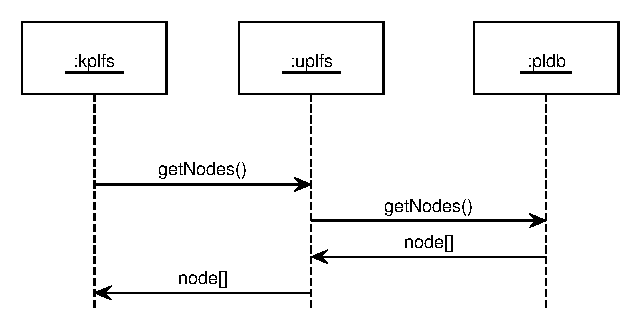
\includegraphics[scale=1.0]{act_-_ls_nodes.eps}
	\caption{Listado de nodos}
	\label{fig:act_-_ls_nodes}
\end{figure}



\section{Listado de slices}

El comando que lanzar�a esta operaci�n seria \texttt{ls /plfs/slices/}, y el
diagrama de sus operaciones es el que se muestra en la figura
\ref{fig:act_-_ls_slices}.

\begin{figure}[h]
	\centering
	\includegraphics[scale=1.0]{act_-_ls_slices.eps}
	\caption{Listado de slices}
	\label{fig:act_-_ls_slices}
\end{figure}



\section{Listado de ficheros compartidos}

El comando que lanzar�a esta operaci�n ser�a \texttt{ls
/plfs/slices/\textless{}slice\textgreater/shared/}, y el diagrama de sus
operaciones es el que se muestra en la figura \ref{fig:act_-_ls_shared}.

\begin{figure}[h]
	\centering
	\includegraphics[scale=1.0]{act_-_ls_shared.eps}
	\caption{Listado de ficheros compartidos}
	\label{fig:act_-_ls_shared}
\end{figure}



\section{Listado de nodos de un slice}

El comando que lanzar�a esta operaci�n ser�a \texttt{ls
/plfs/slices/\textless{}slice\textgreater/nodes/}, y el diagrama de sus
operaciones es el que se muestra en la figura \ref{fig:act_-_ls_slice_nodes}.

\begin{figure}[h]
	\centering
	\includegraphics[scale=1.0]{act_-_ls_slice_nodes.eps}
	\caption{Listado de nodos de un slice}
	\label{fig:act_-_ls_slice_nodes}
\end{figure}



\section{Listado de ficheros no compartidos}

El comando que lanzar�a esta operaci�n ser�a \texttt{ls
/plfs/slices/\textless{}slice\textgreater/nodes/\textless{}node\textgreater/unshared/},
y el diagrama de sus operaciones es el que se muestra en la figura
\ref{fig:act_-_ls_unshared}.

\begin{figure}[h]
	\centering
	\includegraphics[scale=1.0]{act_-_ls_unshared.eps}
	\caption{Listado de ficheros no compartidos}
	\label{fig:act_-_ls_unshared}
\end{figure}



\section{Obtenci�n de un fichero}

El comando que lanzar�a esta operaci�n ser�a, por ejemplo, un \texttt{cat} de
un fichero, ya fuera en \texttt{shared} o \texttt{unshared}, y el diagrama de
sus operaciones es el que se muestra en la figura \ref{fig:act_-_get}.

\begin{figure}[h]
	\centering
	\includegraphics[scale=1.0]{act_-_get.eps}
	\caption{Obtenci�n de un fichero}
	\label{fig:act_-_get}
\end{figure}



\section{Despliegue}

% TODO: desplegar el soft de despliegue si no esta presente y es un nuevo
% nodo?

El comando que lanzar�a esta operaci�n ser�a, por ejemplo, un \texttt{cp} de
un fichero, ya fuera a \texttt{shared} a \texttt{unshared}, y el diagrama de
sus operaciones es el que se muestra en la figura \ref{fig:act_-_put}.

\begin{figure}[h]
	\centering
	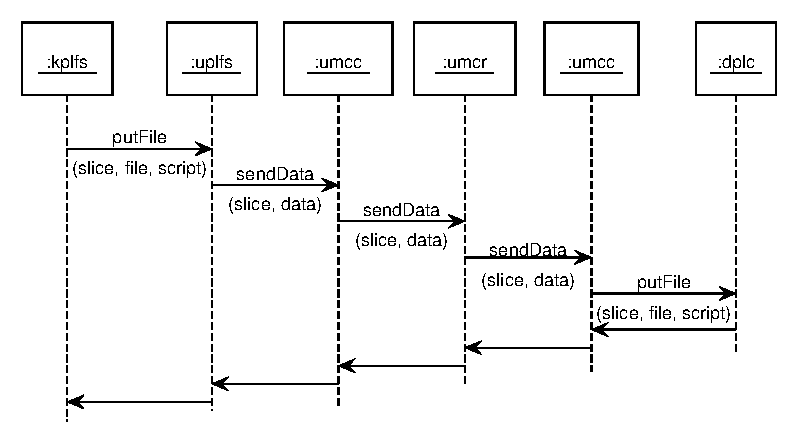
\includegraphics[scale=1.0]{act_-_put.eps}
	\caption{Despliegue}
	\label{fig:act_-_put}
\end{figure}



\section{Adici�n de un nodo a un grupo}

�sta operaci�n se llevar�a a cabo al crear una nueva m�quina virtual en un
nodo donde ya este corriendo \dplc, y el diagrama de sus operaciones es el que
se muestra en la figura \ref{fig:act_-_join}.

\begin{figure}[h]
	\centering
	\includegraphics[scale=1.0]{act_-_join.eps}
	\caption{Adici�n de un nodo a un grupo}
	\label{fig:act_-_join}
\end{figure}



\section{Eliminaci�n de un nodo de un grupo}

�sta operaci�n se llevar�a a cabo al eliminar una m�quina virtual de un nodo
donde ya este corriendo \dplc, y el diagrama de sus operaciones es el que se
muestra en la figura \ref{fig:act_-_delete}.

\begin{figure}[h]
	\centering
	\includegraphics[scale=1.0]{act_-_delete.eps}
	\caption{Eliminaci�n de un nodo de un grupo}
	\label{fig:act_-_delete}
\end{figure}


\pagebreak
\addcontentsline{toc}{chapter}{Bibliograf�a}
\bibliographystyle{plain}
\bibliography{00-plfs}

\end{document}

